%%%%%%%%%%%%%%%%%%%%%%%%%%%%%%%%%%%%%%%%%%%%%%%%%%%%%%%%%%%%%%%%%%%%%%
%     File: ExtendedAbstract_backg.tex                               %
%     Tex Master: ExtendedAbstract.tex                               %
%                                                                    %
%     Author: Andre Calado Marta                                     %
%     Last modified : 27 Dez 2011                                    %
%%%%%%%%%%%%%%%%%%%%%%%%%%%%%%%%%%%%%%%%%%%%%%%%%%%%%%%%%%%%%%%%%%%%%%
% A Theory section should extend, not repeat, the background to the
% article already dealt with in the Introduction and lay the
% foundation for further work.
%%%%%%%%%%%%%%%%%%%%%%%%%%%%%%%%%%%%%%%%%%%%%%%%%%%%%%%%%%%%%%%%%%%%%%

\section{Must-Have Concepts}
\label{sec:must_have_concepts}

This section discusses topics that help understand the technological developments along this thesis project. The developments involve both hardware and software components. As such, there are hardware and software concepts that are important to have before discussing the following chapters.
%
%The candidate will develop an SoC in this project. However, he will not create it from scratch. The candidate will use the \textit{IOb-SoC} as a starting point. Consequently, it is vital to understand how the \textit{IOb-SoC} works beforehand. Studying the RISC-V Instruction set architecture (ISA) is also indispensable. Since the hardware developed in this project will be compatible with the RISC-V ISA.
%Additionally, the RISC-V foundation has created hardware specifications for hardware compatible with RISC-V systems which are essential to know. Furthermore, a necessary concept for this project is an Operating System (OS) boot flow on a RISC-V platform. Lastly, a crucial part when developing a system is its testing and simulation before implementation. Therefore, the author will review the available methods for simulating the developed components.


%%%%%%%%%%%%%%%%%%%%%%%%%%%%%%%%%%%%%%%%%%%%%%%%%%%%%%%%%%%%%%%%%%%%%%
\subsection{The \textit{IOb-SoC} platform}

The \textit{IOb-SoC}~\cite{iob_soc} is a System on a chip (SoC) template that eases the creation of a new SoC. The IObSoC provides a base \textit{Verilog}~\cite{thomas2008verilog} hardware design equipped with an open-source RISC-V processor, an internal SRAM memory subsystem, a UART, and an optional interface to external memory. If the external memory interface is selected, the \textit{IOb-SoC} will include an instruction L1 cache, a data L1 cache and a shared L2 cache. The L2 cache communicates with a third-party memory controller IP (typically a DDR controller) using an \textit{AXI4}~\cite{tidala2018high} master bus.

Figure \ref{fig:bd_original} represents a sketch of the SoC design. This design is valid at the start of this project. During the hardware development the \textit{IOb-SoC} original template suffered a few alterations.

\begin{figure}[!ht]
  \centering
  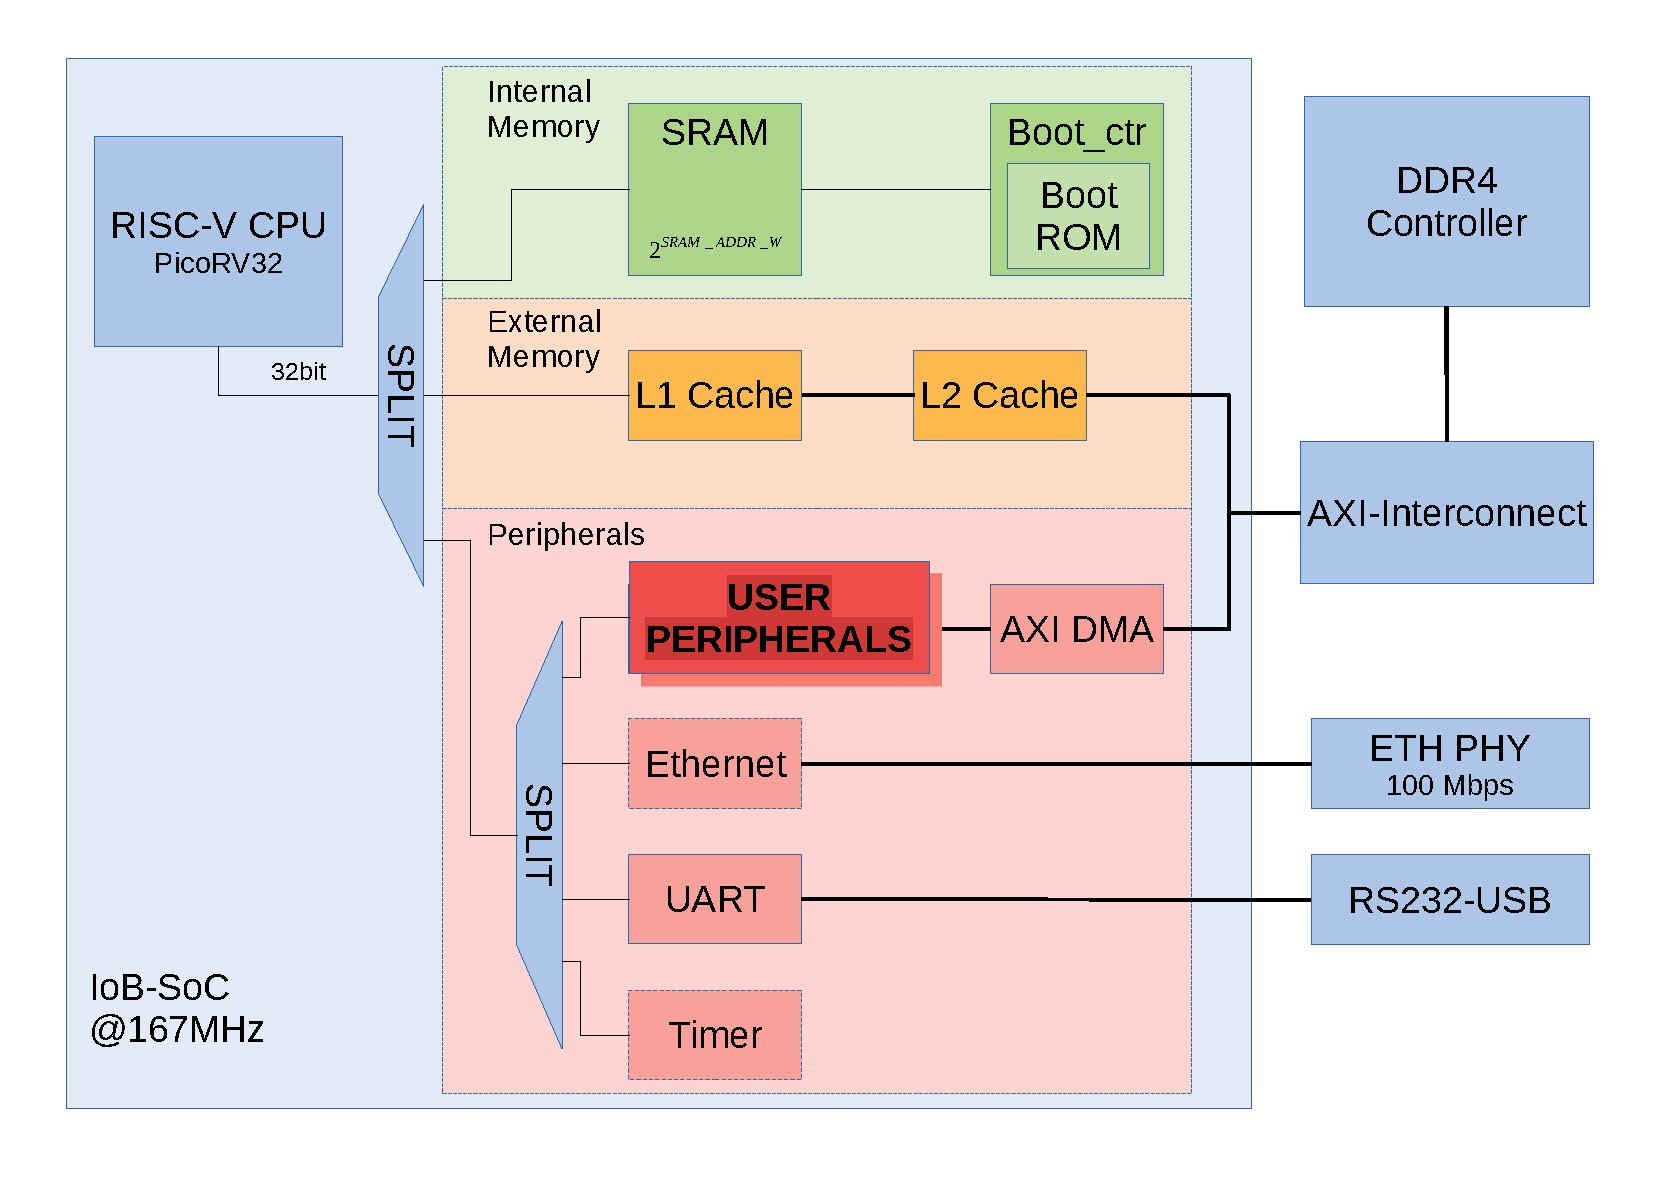
\includegraphics[width=\linewidth]{../images/bd_original.pdf}
  \caption{\textit{IOb-SoC} sketch.}
  \label{fig:bd_original}
\end{figure}

\textit{IOb-SoC} currently supports two FPGA board models: the \textit{Xilinx Kintex UltraScale KU040 Development Board} and the \textit{Cyclone V GT FPGA Development Kit}.

%\subsubsection{\textit{IOb-SoC} \textit{Makefiles}}
The main \textbf{\textit{Makefile}} in \textit{IOb-SoC} is located at the \textit{IOb-SoC} root directory. The main \textit{Makefile} contains targets that call other \textit{Makefiles} and sets the values for the default frequency, baud rate, FPGA board used and simulator used. The \textit{Makefiles} the main one can call are at the \textit{IOb-SoC} FPA boards, simulators, firmware, "PC" emulation or documentation directory. Each directory in \textit{IOb-SoC} contains a "*.mk" file which holds "make" variables and targets that complement the \textit{Makefiles}. The \textit{IOb-SoC} \textit{Makefiles} can include only the "*.mk" they need.

%When executing the command \textit{"make sim-run"} the computer will run the "run" target of the \textit{Makefile} in the default simulator directory. The simulator \textit{Makefile} will include the "simulator.mk", "hardware.mk" and "config.mk" files. The "simulator.mk" file is common to all simulators. Both FPGAs and simulators \textit{Makefiles} include the "hardware.mk" file. The "hardware.mk" file includes all the hardware modules that the SoC uses. Lastly, the "config.mk" is located at the \textit{IOb-SoC} root directory and all \textit{Makefiles} use it. The "config.mk" defines the "make" variables that are important for hardware and software, for example which peripherals the SoC contains.

A \textit{IOb-SoC} \textbf{peripheral} should have the following "*.mk" files to integrate it into \textit{IOb-SoC}:
\begin{itemize}
    \item the "PERIPHERAL\_REPO/hardware/hardware.mk" so the user can add the peripheral hardware modules to the SoC.
    \item the "PERIPHERAL\_REPO/software/embedded/embedded.mk" allows the user to use the peripheral firmware drivers.
    \item the "PERIPHERAL\_REPO/software/pc-emul/pc-emul.mk" permits emulating the peripheral behaviour in the user's computer.
\end{itemize}

The \textit{IOb-SoC} \textbf{request bus} comprises a valid bit, an address signal, a data signal and a strobe signal. The hardware sets the valid bit to '1' when it wants to execute a request and has already defined the other signals. The address signal indicates the register that the request is targeting. Figure \ref{fig:req_bus} shows how the \textit{IOb-SoC} distributes the signals in the request bus. Furthermore, figure \ref{fig:req_bus} also represents the bits equivalent to each signal when the address width and data width are 32 bits. The address and data width in \textit{IOb-SoC} are 32-bit by default.

\begin{figure}[!ht]
    \centering
    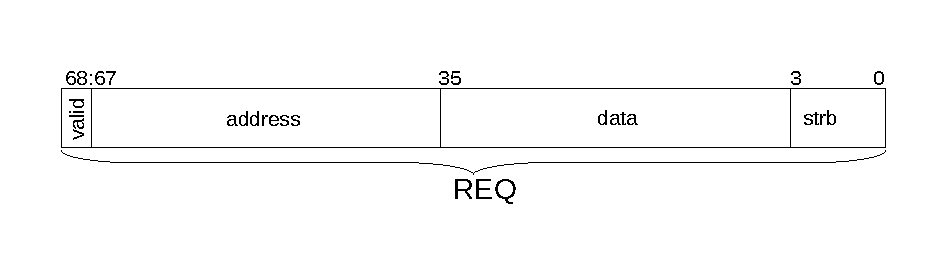
\includegraphics[width=\linewidth]{../images/req_bus.pdf}
    \caption{Request bus with address and data width equal to 32 bits.}
    \label{fig:req_bus}
\end{figure}

The \textit{IOb-SoC} \textbf{response bus} contains a ready bit and a data signal. The hardware sets the ready signal to high when the component that made the request can receive the response. The data signal is the response data to the request made. For example, if the CPU wants to read the value in a register at address "x", the data in the response bus will be the data on register "x". Figure \ref{fig:resp_bus} shows how the request signal is composed when the address and data width are 32 bits.

\begin{figure}[!ht]
    \centering
    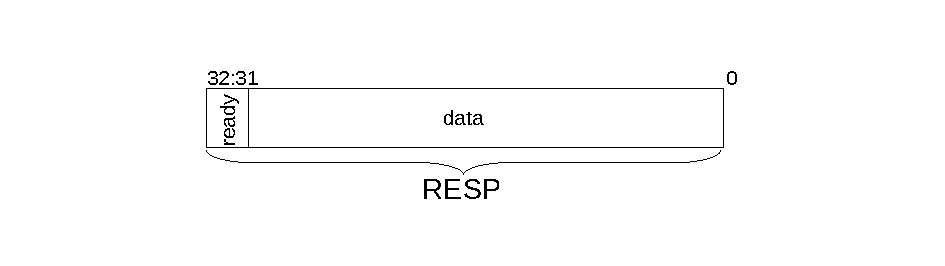
\includegraphics[width=\linewidth]{../images/resp_bus.pdf}
    \caption{Response bus with address and data width equal to 32 bits.}
    \label{fig:resp_bus}
\end{figure}

The \textbf{\textit{iob-split}} is simply a configurable demultiplexer (DEMUX). The developer can configure it when he instantiates the \textit{iob-split} hardware module. The developer can change the size of the DEMUX and the selection bits through N\_SLAVES and P\_SLAVES, respectively. N\_SLAVES corresponds to the number of slaves. Developers can also interpret N\_SLAVES as the number of the DEMUX outputs. P\_SLAVES indicates the slave select word most significant bit (msb) position. In other words, P\_SLAVES is the position of the msb of the DEMUX selection bits. Equation \ref{eq:number_bits} calculates the number of the selection bits.

\begin{equation}
    \label{eq:number_bits}
    Nb = log_2(N\_SLAVES)+(log_2(N\_SLAVES)==0)
\end{equation}

The \textbf{\textit{iob-merge}} works similar to the \textit{iob-split} but instead of being a DEMUX it is a configurable multiplexer (MUX). Meaning that instead of having multiple outputs and one input, it has multiple inputs and one output. N\_SLAVES indicates the number of inputs, and P\_SLAVES chooses the selection bits.

The \textit{IOb-SoC} \textbf{bootloader} is the first firmware to run on the SoC. Figure \ref{fig:boot_flow} represents a flow chart of the bootloader firmware behaviour.

\begin{figure}[!h]
    \centering
    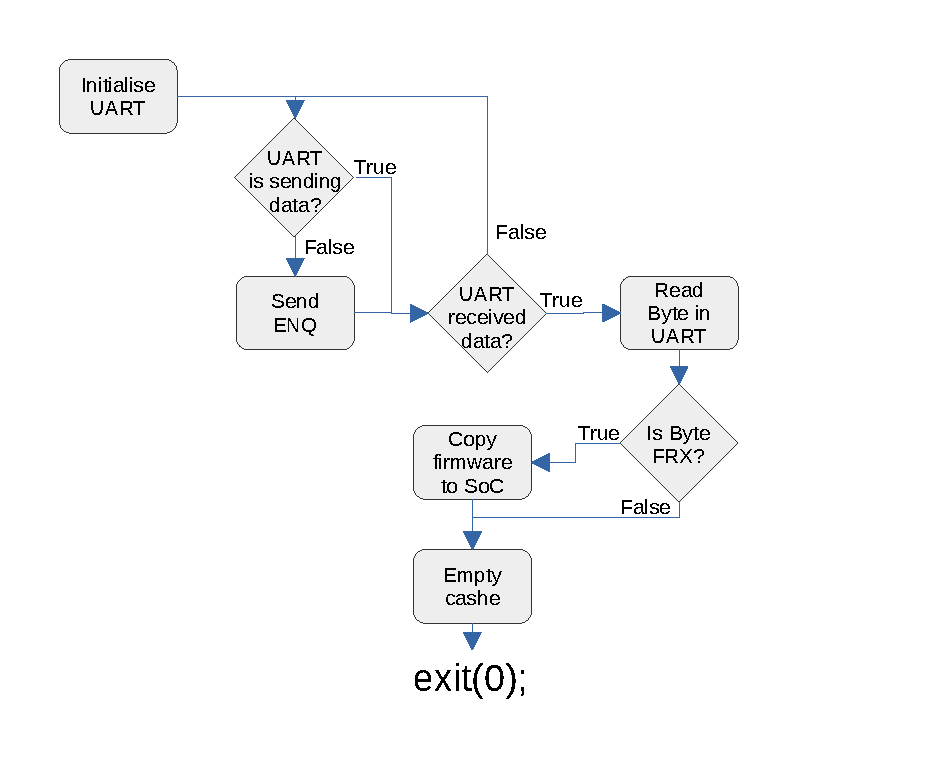
\includegraphics[width=\linewidth]{../images/boot_flow.pdf}
    \caption{Bootloader firmware flow chart.}
    \label{fig:boot_flow}
\end{figure}

%%%%%%%%%%%%%%%%%%%%%%%%%%%%%%%%%%%%%%%%%%%%%%%%%%%%%%%%%%%%%%%%%%%%%%
\subsection{\textit{RISC-V}}

\textit{RISC-V}~\cite{asanovic2014instruction} is a free-to-use, open-source RISC Instruction set architecture (ISA). The \textit{RISC-V} ISA defines the instructions which a \textit{RISC-V} compatible CPU can interpret. Those instructions represent the software written in C, Python, or any other programming language to be executed by the CPU.

The \textit{RISC-V} ISA is divided in two main volumes. The "RISC-V Instruction Set Manual Volume I"~\cite{riscv_unprivilege} contains the specification for the \textbf{unprivileged} instructions. The unprivileged instructions are instructions that do not need any special permission to execute. The "RISC-V Instruction Set Manual Volume II"~\cite{riscv_privilege} defines the \textit{RISC-V} \textbf{privilege} levels and the instructions that take advantage of them. Table \ref{tab:riscv_privilege_levels} shows the privilege levels currently defined in the \textit{RISC-V} specification. Developers must implement all three privilege levels to run a Unix-like OS.

\begin{table}[!ht]
  \centering
  \begin{tabular}{|l|l|l|l|}
  \hline
  \textbf{Level} & \textbf{Name}    & \textbf{Abbreviation} \\ \hline
  0              & User/Application & U                     \\ \hline
  1              & Supervisor       & S                     \\ \hline
  2              & Reserved         &                       \\ \hline
  3              & Machine          & M                     \\ \hline
  \end{tabular}
  \caption{\textit{RISC-V} privilege levels.}
  \label{tab:riscv_privilege_levels}
\end{table}

The \textit{RISC-V} \textbf{CLINT} specification~\cite{clint_riscv_spec} describes the hardware registers of a Core-local Interrupt Controller (CLINT) compatible with \textit{RISC-V} platforms. The hardware uses the CLINT to generate the inter-processor software and timer interrupts.

The \textit{RISC-V} systems use the Platform-Level Interrupt Controller (\textbf{PLIC}) hardware to gather various device interrupts and have only one external interrupt line per \textit{RISC-V} Hart context. A PLIC that claims to be a PLIC-Compliant standard PLIC has to follow the \textit{RISC-V} PLIC specification~\cite{plic_riscv_spec}.

In the \textit{RISC-V} Platform Specification~\cite{riscv_platform_specification} it is defined that every embedded OS is required to have a UART port implementation that is register-compatible with the industry standard \textbf{\textit{UART16550}}. The \textit{UART16550} already existed for a long time and developers often use it to connect to an RS-232 interface.

The Supervisor Binary Interface (\textbf{SBI}) specification~\cite{sbi_riscv_spec} defines an abstraction for platform-specific functionalities. Figure \ref{fig:riscv_sbi} illustrates the purpose of the SBI in a system executing an OS like the one the author is going to develop in this thesis.

\begin{figure}[!h]
    \centering
    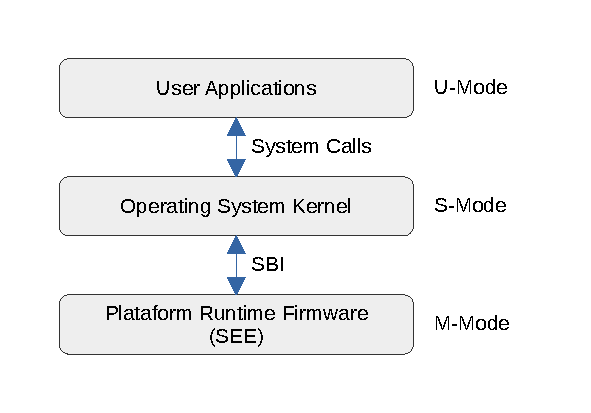
\includegraphics[width=0.8\linewidth]{../images/riscv_sbi.pdf}
    \caption{\textit{RISC-V} system running an OS.}
    \label{fig:riscv_sbi}
\end{figure}

\textbf{\textit{OpenSBI}} is the recommended interface between a platform-specific firmware running in M-mode and a general-purpose OS executing in S-mode.

Figure \ref{fig:linux_boot_flow} shows the various stages a \textit{RISC-V} system has to pass through to fully \textbf{boot a Linux OS}.

\begin{figure}[!h]
  \centering
  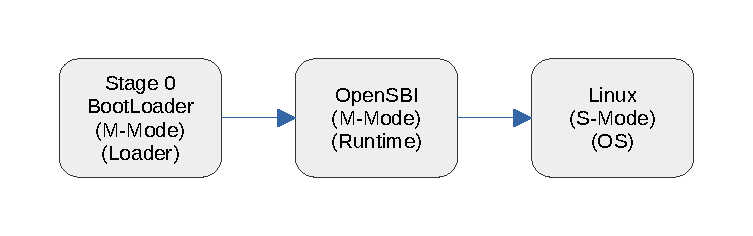
\includegraphics[width=0.9\linewidth]{../images/linux_boot_flow.pdf}
  \caption{Stages of the Linux boot on \textit{RISC-V} on a minimal system.}
  \label{fig:linux_boot_flow}
\end{figure}

\subsection{Open Source Verification tools}
Verification tools are essential when developing hardware or software components. Verification tools allow developers to simulate their work before implementing it in real hardware and test new features in a safe environment where the SoC implementation does not use hardware components. In this thesis project, the author has to simulate hardware logic components and platform-independent software. For that purpose there are three types of verification software that the author is going to use: a \textbf{functional} emulator, a \textbf{cycle-accurate} simulator and an \textbf{event-driven} simulator.

Developers can use cycle-accurate and event-driven simulators to simulate the hardware logic designs. \textbf{Cycle-accurate}  simulators are suitable for complex hardware designs. An example of a cycle-accurate simulator would be \textit{Verilator}. \textbf{Event-driven} simulators are adequate for small hardware designs. An example of an event-driven simulator would be \textit{Icarus Verilog}.

A \textbf{functional} emulator translates the instructions that were supposed to run on the target architecture to instructions that run on the host CPU. The advantage of using a functional emulator is that it is way faster than the other emulation types. An example of a functional emulator would be \textbf{\textit{QEMU}}~\cite{bellard2005qemu}.

\section{Existing Embedded Technologies}
\label{sec:existing_embedded_technologies}
There already exists embedded microcontrollers capable of running Linux. However, most of them are closed source. For example from Arm Holdings (Arm ®), Andes Technology and SiFive. Andes Technology and SiFive are members of the \textit{RISC-V} community and have contributed with open-source components. 

Built upon the \textit{RISC-V} open-source ISA, various open-source CPU designs have emerged. An \textit{application processor} is needed to run a Linux OS. \textit{Application processors} have the necessary CSR, support M+S+U privilege modes, and support atomic instructions. 

An open-source CPU solution would be either the \textit{CVA6}~\cite{zaruba2019cost} (previously known as Ariane), \textit{BOOM}~\cite{zhaosonicboom} or \textit{VexRiscv}~\cite{vexriscv}. The \textit{CVA6} is a 6-stage, single issue, in-order CPU which can execute either the 32-bit or 64-bit \textit{RISC-V} instruction set. The Berkeley Out-of-Order \textit{RISC-V} Processor (\textit{BOOM}) is a superscalar Out-of-Order processor executing the RV64GC variant of the \textit{RISC-V} ISA. The \textit{VexRiscv} CPU is a 32-bit Linux Capable \textit{RISC-V} CPU written in the \textit{SpinalHDL}~\cite{papon2017spinalhdl}.